% Created 2021-10-05 ter 11:09
% Intended LaTeX compiler: pdflatex
\documentclass[11pt]{article}
\usepackage[utf8]{inputenc}
\usepackage[T1]{fontenc}
\usepackage{graphicx}
\usepackage{grffile}
\usepackage{longtable}
\usepackage{wrapfig}
\usepackage{rotating}
\usepackage[normalem]{ulem}
\usepackage{amsmath}
\usepackage{textcomp}
\usepackage{amssymb}
\usepackage{capt-of}
\usepackage{hyperref}
\usepackage{braket}
\author{Filipe Gonçalves Jacinto}
\date{04 de Outubro de 2021}
\title{Implementação do Método variacional para resolver o Oscilador Harmônico e o modelo de Kronig-Penney}
\hypersetup{
 pdfauthor={Filipe Gonçalves Jacinto},
 pdftitle={Implementação do Método variacional para resolver o Oscilador Harmônico e o modelo de Kronig-Penney},
 pdfkeywords={},
 pdfsubject={},
 pdfcreator={Emacs 27.2 (Org mode 9.5)}, 
 pdflang={English}}
\begin{document}

\maketitle
\tableofcontents


\section{Introdução:}
\label{sec:org9206440}
Uma das equações mais importantes da mecânica quântica é a Equação de Schoroedinger Independente do Tempo(ESIT) descrita na equação \ref{eq1}.Através da ESIT é possível calcular o espectro de  energia do sistema. Contudo, resolver esta equação não é algo trivial, e a maior parte dos potencias não tem solução analítica e portanto se faz necessário o uso de métodos alternativos como o variacional para resovler esta equação numéricamente.


\begin{equation}
\label{eq1}
\hat{H}
\ket{\psi} = E \ket{\psi}
\end{equation}

Um dos problemas mais importantes da mecânica quântica é o  potencial do oscilador harmônico (equação \ref{eq2}), este sistema tem solução analítica bem conhecida descrito na equação (\ref{eq3}) e pode ser utilizado para testar a eficiência do método variacional para resolver a ESIT.

\begin{equation}
\label{eq2}
V(x) = \frac{1}{2} m \omega^2 \left(x - \frac{a}{2}\right)^2
\end{equation}

\begin{equation}
\label{eq3}
E = \left(n + \frac{1}{2}\right) \hbar \omega
\end{equation}

Em seguida de forma a estudar um potencial mais complicado, o método variacional será utilizado para calcular o dispersão de energia \(E(K)\) no modelo de kronig Penney que é descrito no potencial periódico da equação \ref{eq4}. Este modelo é uma simplificação e descreve um cristal unidimensional perfeito mostrando o comportamento das bandas de energia nesse sistema. Além disso, este sistema também possui solução analítica e portanto permite a comparação com o resultado obtido por meio do
método variacional.

\begin{equation}
\label{eq4}
V(x)= V(x+a) =\[ \begin{cases}
      0 & 0 < x < \frac{a -b}{2}\\
      V_0 & \frac{a -b}{2}\leq x\leq  \frac{a+b}{2}\\
      0 & \frac{a+b}{2} < x < a
   \end{cases}
\]
\end{equation}


Desse modo, este trabalho irá estudar por meio do método variacional os problemas do Oscilador Harmônico quântico e o modelo de Kroning Penney . Para isso, será discutido a base teórica e o algoritmo utilizado para resolver de forma numérica a equação de Schoroedinger referente a cada potencial utilizando o método variacional.



\section{Metodologia:}
\label{sec:orgb3ef600}
\subsection{Método Variacional:}
\label{sec:orga51ca98}
O método variacional é uma forma de calcular a energia do estado fundamental e de alguns dos primeiros estados excitados utilizando o princípio variacional.Para isso, o método utiliza um conjunto de funções que formam uma base para o sistema denominadas como funções teste. Então expandindo a função de onda \(\ket{\psi}\) usando uma superposição de autoestados da base, pode-se resolver o problema através da base escolhida.
\begin{equation}
\label{eq5}
\ket{\psi} = \sum_{n} C_n \ket{\psi_n}
\end{equation}
Através de uma algebra simples pode-se rescrever o problema na forma matricial, o que é bem útil do ponto de vista computacional já que o torna o sistema mais simples de tratar modo geral. A partir da equação de autovalor pode-se utilizar a expansão proposta anteriormente para para obter a equação \ref{eq8}.

\begin{equation}
\label{eq6}
\hat{H} \ket{\psi_n} = E_n \ket{\psi_n}
\end{equation}
\begin{equation}
\label{eq7}
\sum_{n} c_n \braket{\psi_m|\hat{H} |\psi_n} = \sum_{n} c_n E_n \braket{\psi_m|\psi_n}
\end{equation}
\begin{equation}
\label{eq8}
\sum_{n} c_n H_{mn}  = \sum_{n} c_n E_n S_{mn}
\end{equation}
Como vamos utilizar bases normalizadas  \(S_{mn} = \delta_{mn}\), ou seja a matriz identidade. Seguindo em frente, a hamiltoniana do problema consiste em uma parte cinética (\(\hat{T}\)) e a parte do potencial (\(\hat{V}\)). E nesta parte está o maior desafio do problema que é construir a matriz hamiltoninana \(H_{mn}\) a partir das matrizes da energia cinética (\(T_{mn}\)) e do potencial (\(V_{mn}\)).

Para escrever a matriz hamiltoniana é necessário escrever os operadores separadamente, e em seguida entender como cada elemento da matriz será calculado à partir de cada operador. As equações 9 até 13 mostram como construir a matriz \(H_{mn}\) elemento a elemento.
\begin{equation}
\hat{H} = \hat{T} + \hat{V} = -\frac{1}{2}\frac{d^2}{dx^2} + \hat{V}(x)
\end{equation}
\begin{equation}
\braket{\psi_m|\hat{H} |\psi_n} = \braket{\psi_m|\hat{T} |\psi_n} + \braket{\psi_m|\hat{V} |\psi_n}
\end{equation}
\begin{equation}
T_{mn} = \braket{\psi_m|\hat{T} |\psi_n} = \int_{-\infty}^{~\infty} \psi_m^{*}(x) \left(-\frac{1}{2} \frac{d^2}{dx^2}\right) \psi_n(x) dx
\end{equation}
\begin{equation}
V_{mn} = \braket{\psi_m|\hat{V} |\psi_n} = \int_{-\infty}^{~\infty} \psi_m^{*}(x)  \hat{V}(x)  \psi_n(x) dx
\end{equation}
\begin{equation}
H_{mn} = T_{mn} + V_{mn}
\end{equation}

Após construir a matriz hamiltoniana corretamente  basta resolver o problema de auto valor. Para isto, existem varias bibliotecas ja implementadas. Neste trabalho o pacote \texttt{scipy.linalg} e \texttt{numpy.linalg}  disponíveis na linguagem Python.

\subsection{Algortimo:}
\label{sec:org98dc5eb}

\begin{enumerate}
\item Escolher qual o potencial será resolvido;
\item Escolher uma base para o problema, aqui serão utilizadas duas bases escritas nas equações \ref{eq14} e \ref{eq15} onde \(K_n = \frac{2 \pi}{n}\), no caso do problema do potencial de Kronig-Penney é necessário utilizar o teorema de Bloch (equação \ref{eq16}) o que implica que levando em conta um potencial periódico a solução de uma célula unitária é corrigida apenas por um fator de fase e portanto só é necessário resolver a equação dentro de uma única célula unitária;
\item Calcula-se  os valores do potencial e da base no intervalo;
\item Contrói-se a matriz do integrando utilizando a equação \ref{eq18};
\item Integra-se elemento a elemento as matrizes \(T_{mn}\) e \(V_{mn}\) utilizando um pacote de sua preferência, neste caso foi utilizado a biblioteca de integração do pacote  \texttt{scipy} em específico o método de Simpson;
\item Soma-se as duas matrizes para construir \(H_{mn}\);
\item Basta agora utilizar um pacote de algebra linear para resolver o problema de autovalor.
\end{enumerate}

\begin{equation}
\label{eq14}
\psi_n(x) = \sqrt{\frac{2}{a}} \sin\left({\frac{n \pi x}{a}}\right), n = 0,1,2,...
\end{equation}


\begin{equation}
\label{eq15}
\psi_n(x) = \frac{1}{\sqrt{a}} \exp(i K_n x), n = 0,\pm 1,\pm 2,...
\end{equation}
\begin{equation}
\label{eq16}
 \psi_{K,n} = \exp{(iKx)} u_n(x)
\end{equation}



\begin{equation}
\psi_n = \begin{pmatrix}
  \psi_n(0) \\
  \psi_n(h) \\
  \psi_n(2h) \\
   ... \\
  \psi_n(a) \\
 \end{pmatrix};
V(x) = \begin{pmatrix}
V(0) \\
V(h) \\
V(2h) \\
... \\
V(3h) \\
\end{pmatrix}
\end{equation}


\begin{equation}
\label{eq18}
\psi_m^* \hat{O} \psi_n = \begin{pmatrix}
  \psi_m^*(0) ~\hat{O}~ \psi_n(0) \\
  \psi_m^*(h) ~\hat{O}~ \psi_n(h) \\
  \psi_m^*(2h)~\hat{O}~ \psi_n(2h) \\
   ... \\
  \psi_m^*(a) ~\hat{O}~ \psi_n(a) \\
 \end{pmatrix};
\end{equation}


\section{Resultados e Discussão:}
\label{sec:org001c0ad}
\subsection{Oscilador Harmônico Quântico:}
\label{sec:orgf1b9b10}
O algoritmo descrito na seção anterior foi então utilizado para calcular as energia \(E_n\) do oscilador harmônico, como esperado os primeiros níveis de energia são bem descritos pelo método variacional, contudo perde-se consideravelmente a precisão a partir de \(n=4\) como pode-se ver pela Tabela 1.

A Figura 1 mostra o plot das densidades de probabilidade dos primeiros quatro níveis de energia, dessa forma pode-se compara-los as funções de onda geradas pelos polinômio de Hermite apresentadas na Figura 2. Pode-se ver que os resultados obtidos pelo método variacional concordam bem com os resultados obtidos de forma analítica.

\begin{table}[htbp]
\caption{Valores de energias calculados utilizando a base do potential quadrado infinito e os valores teóricos determinados de acordo com a equação \ref{eq2}.}
\centering
\begin{tabular}{rrrr}
\hline
n & Base & Teórico & \%\(\epsilon\)\\
\hline
1 & 25.0032 & 25.0 & 0.01284\\
2 & 75.0236 & 75.0 & 0.03147\\
3 & 125.1766 & 125.0 & 0.14135\\
4 & 176.0078 & 175.0 & 0.57589\\
5 & 228.9984 & 225.0 & 1.77708\\
6 & 286.5936 & 275.0 & 4.21586\\
7 & 351.3244 & 325.0 & 8.09982\\
\hline
\end{tabular}
\end{table}


\begin{figure}[htbp]
\centering
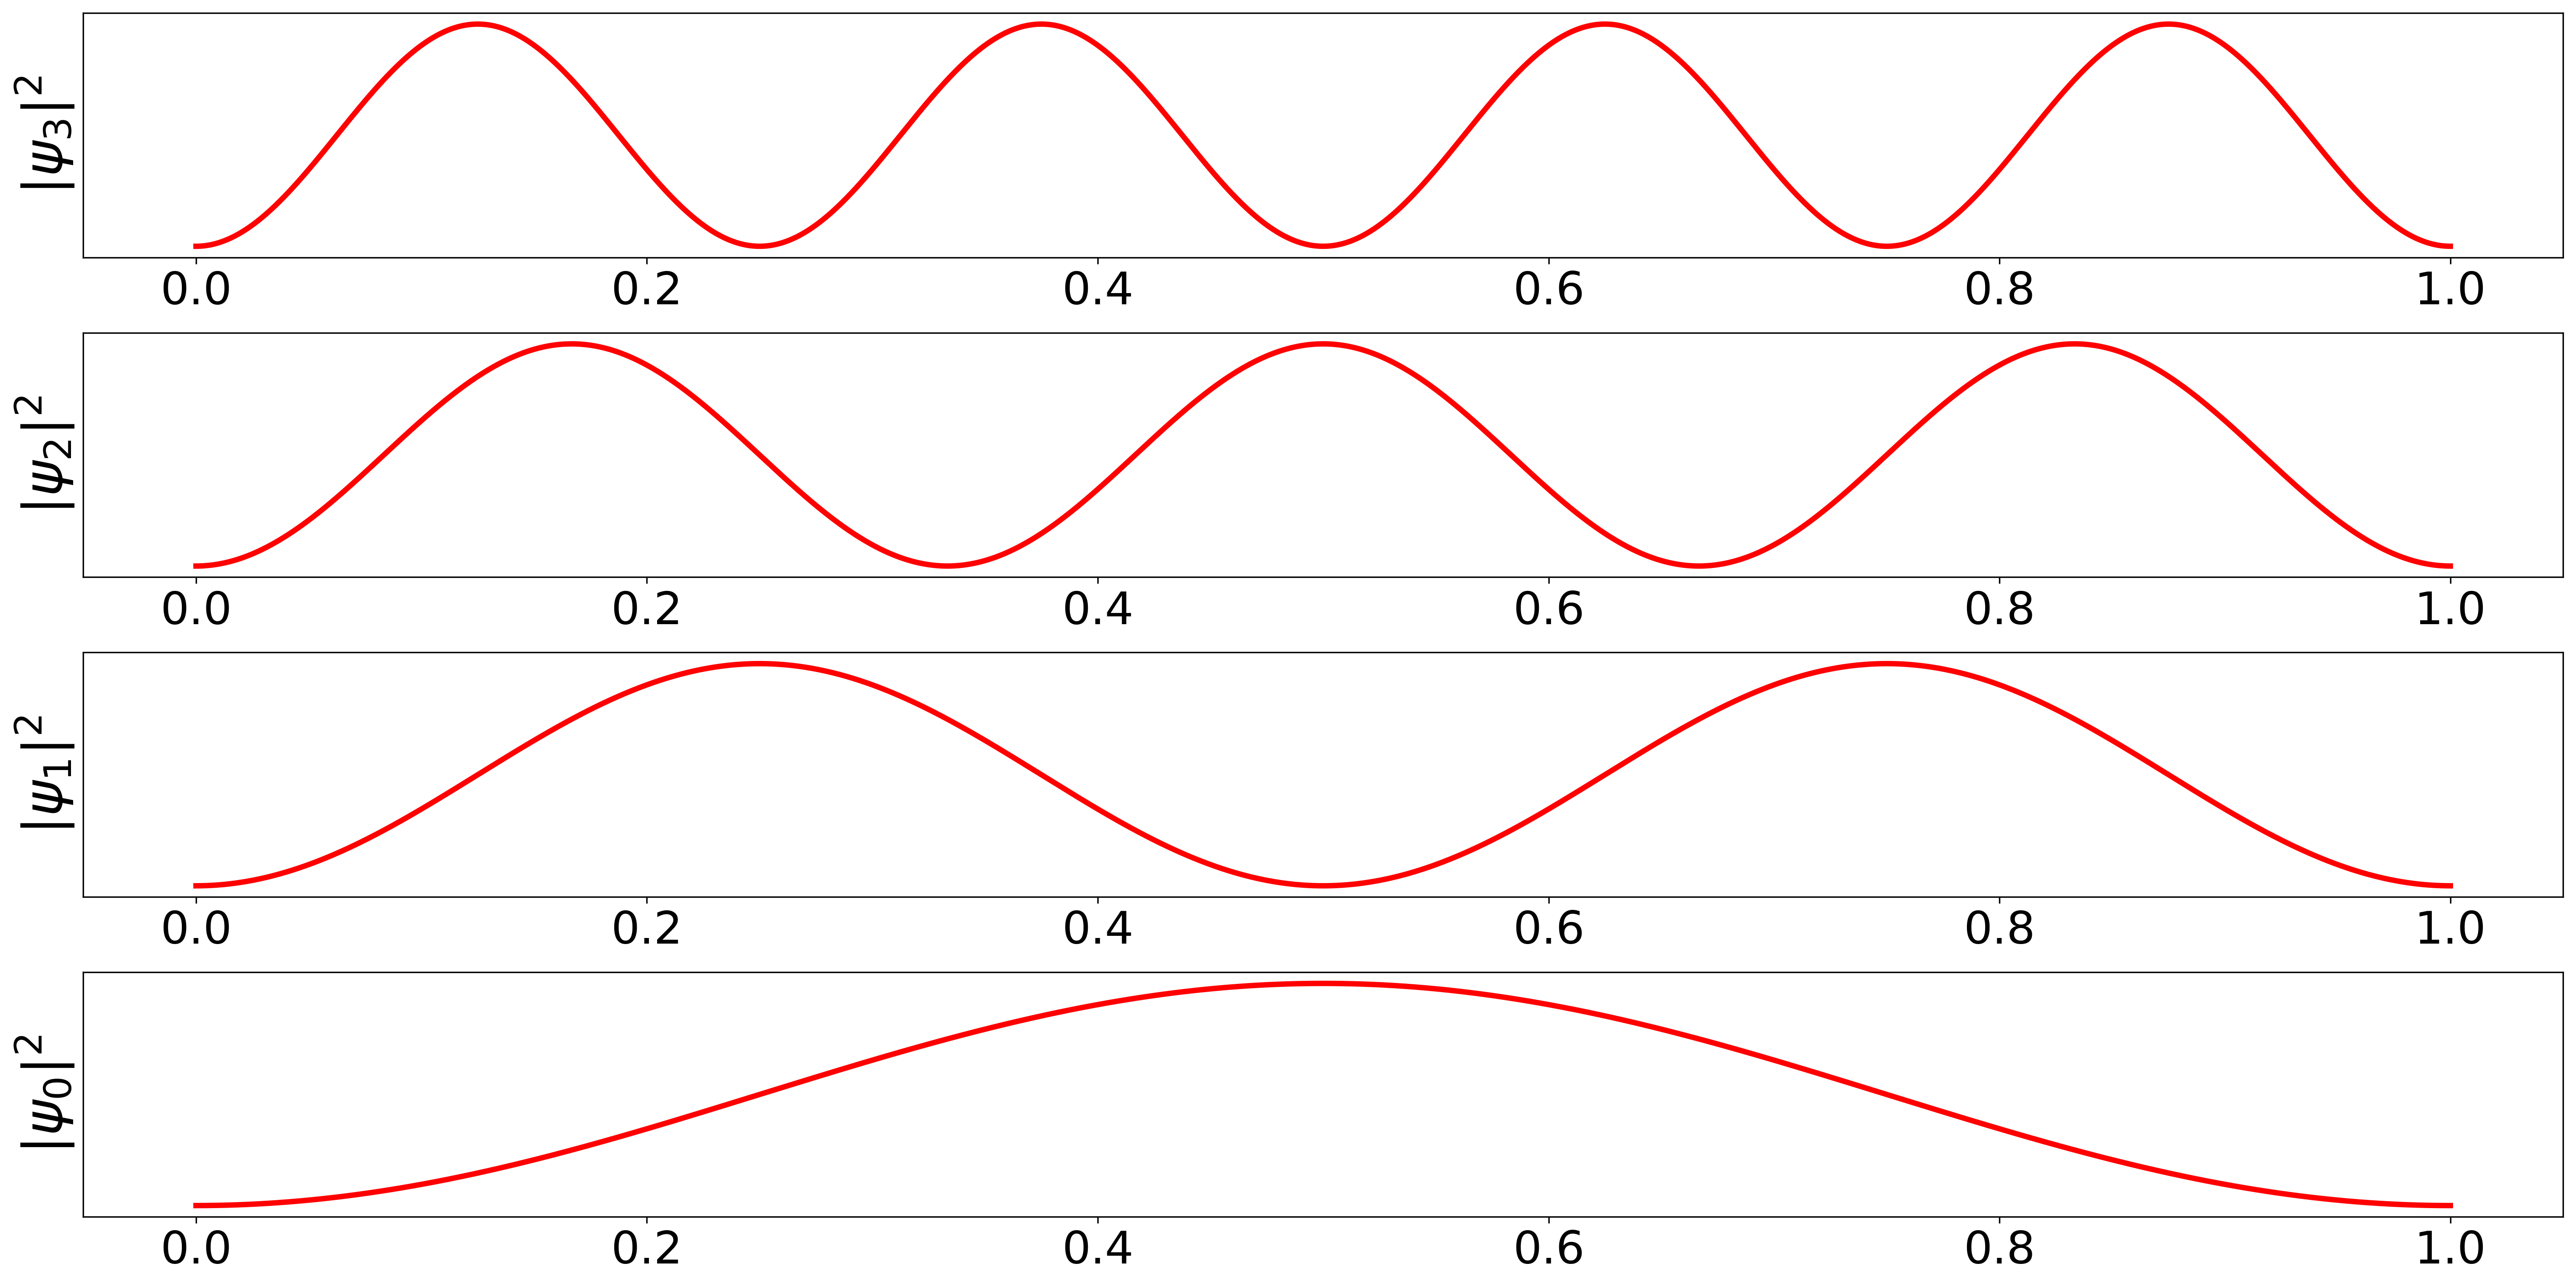
\includegraphics[width=300]{./wavefunction.png}
\caption{Densidade de probabilidade para os quatro primeiros níveis de energia do oscilador harmônico obtidos utilizando o método varicional.}
\end{figure}

\begin{figure}[htbp]
\centering
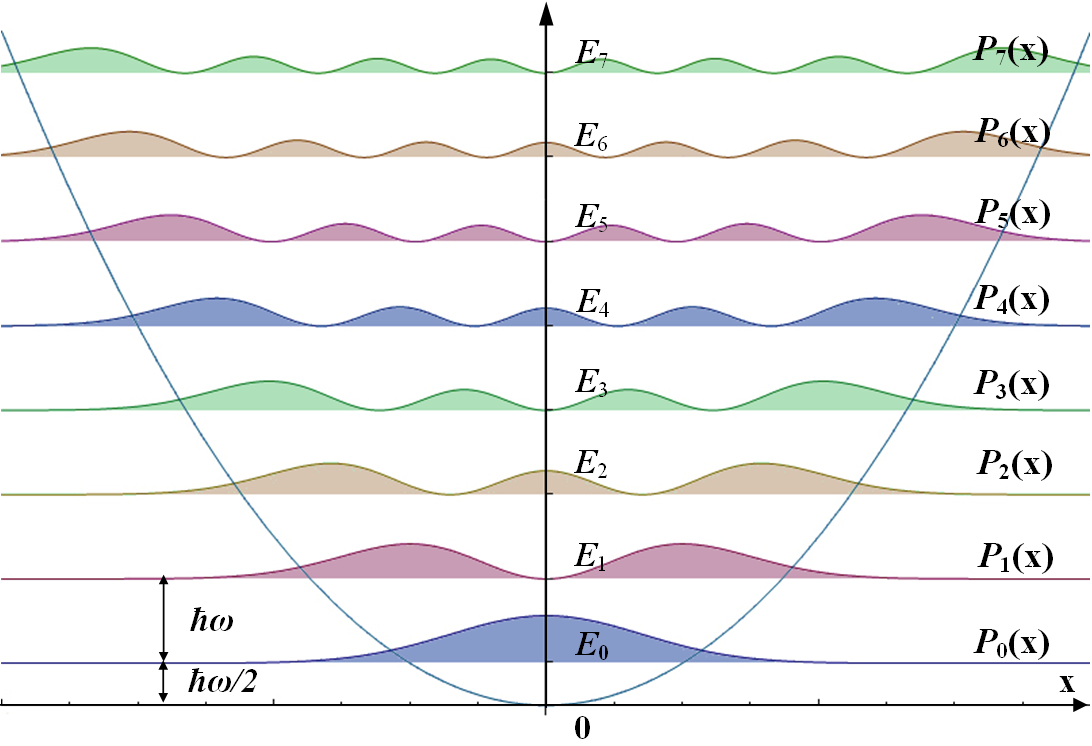
\includegraphics[width=250]{./probability-density.png}
\caption{Densidade de probabilidade para os oito primeiros níveis de energia do oscilador harmônico obtidos de forma analítica.}
\end{figure}

\subsection{Modelo de um sólido 1D:}
\label{sec:org4627ec0}
O modelo de um sólido 1D como dito anteriormente é descrito pelo modelo de Kronig-Penney utilizando um potencial periódico e o teorema de Bloch. Este modelo simplificado é importante porque deixa claro características do comportanto dos elétrons em um potencial periódico em uma dimensão, como se poder ver pela Figura 3, onde ajustando o tamanho \(a\) da barreira de potencial pode-se alterar a dispersão de energia \(E(K)\).

Ao analisar a dispersão de energia na Figura 3 pode-se notar também à presença de \emph{bandgaps} ou seja regiões onde não existem estados acessíveis para estes elétrons. Observe que ao aumentar o tamanho da barreira do potencial periódico aumenta também o tamanho dos \emph{bandgaps} de energia.


\begin{figure}[htbp]
\centering
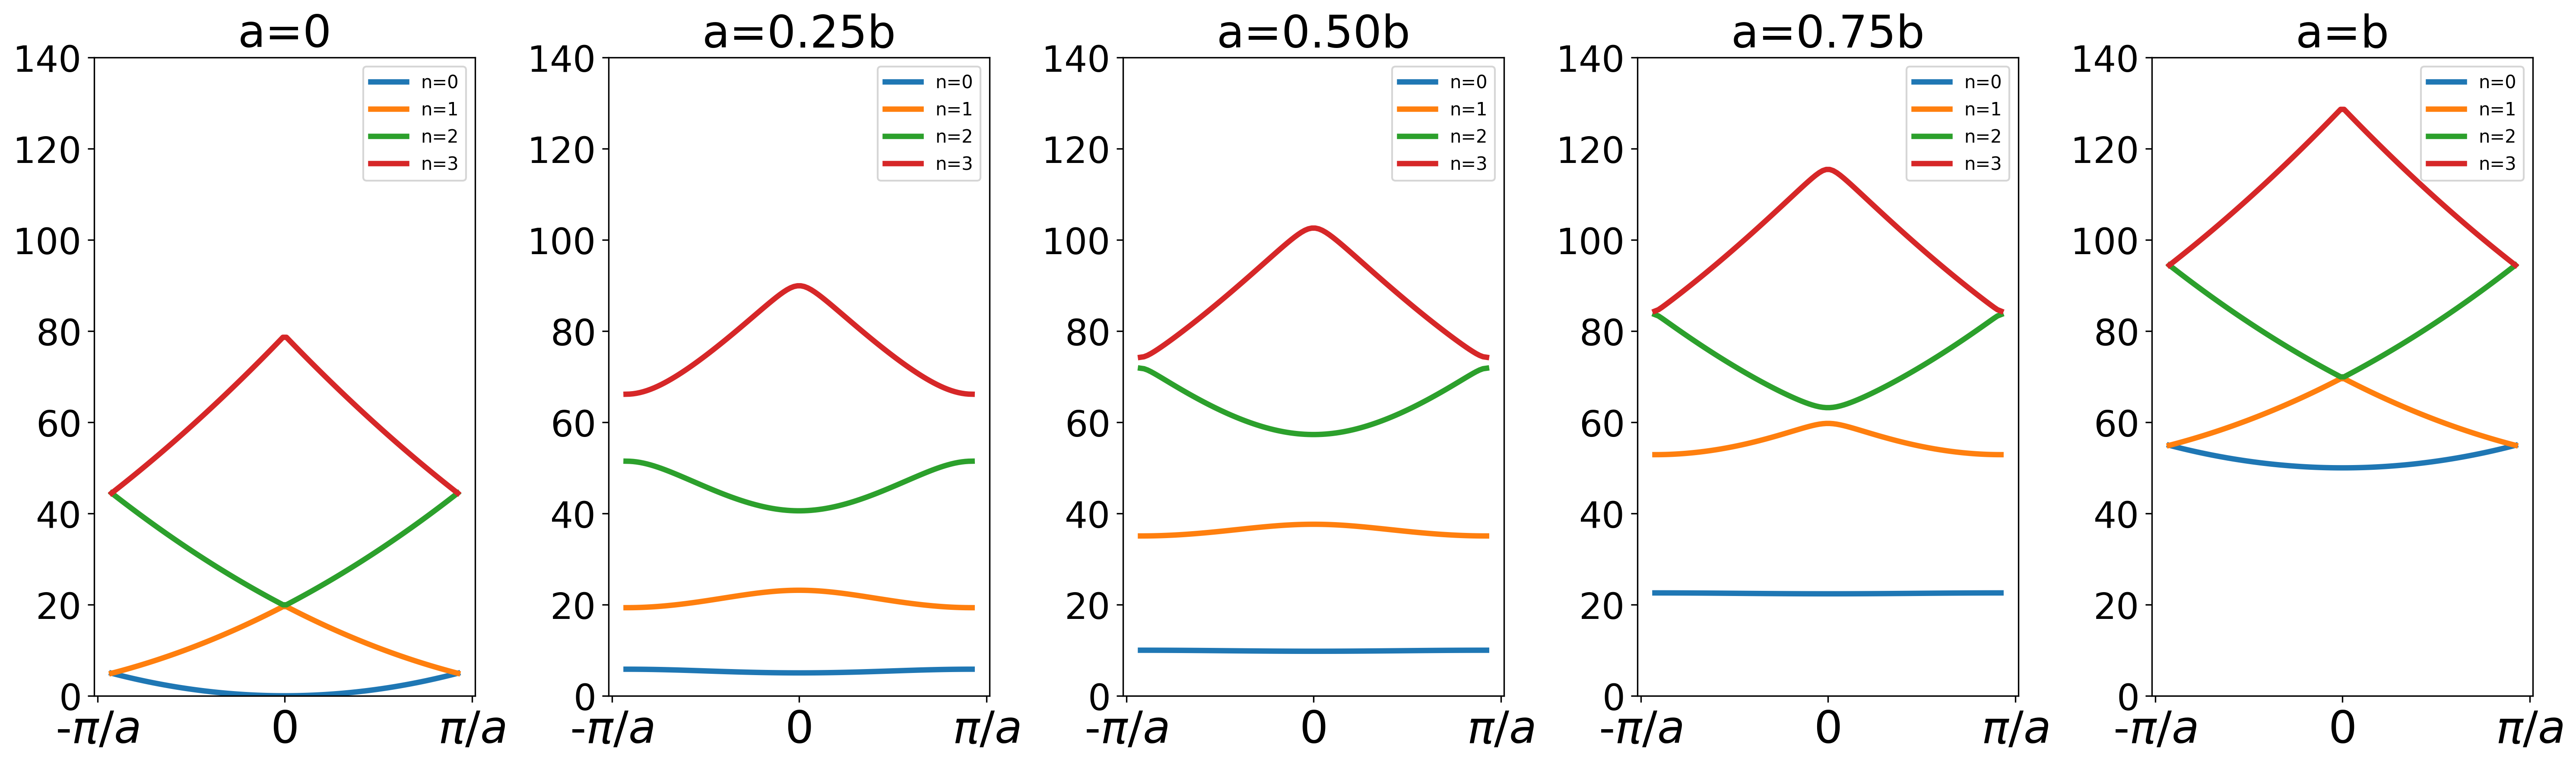
\includegraphics[width=400]{./bands.png}
\caption{Dispersão de energia \(E(K)\) dos primeiros quatro níveis de energia do modelo de Kronig-Penney para um sólido unidimensional.}
\end{figure}
\end{document}
